\setcounter{section}{0}
\section{Lecture 1: Introduction, Degrees of Freedom \& Lagrangian Dynamics}

\subsection{Introduction}

Our goal is to study the dynamics in classical systems ("dynamical systems"). For example, consider a particle moving in 3D, a dynamical system with a dynamical variable $\mathbf{r}$.

\begin{align*}
    \mathbf{r} &= (x_1, x_2, x_3) = \text{position} \\
    \dot{\mathbf{r}} &= \mathbf{v} \\
    \ddot{\mathbf{r}} &= \mathbf{a} 
\end{align*}

\begin{definition}[Dynamical Variables]
    A set of continuous parameters which uniquely specify the state of the system.
\end{definition}

For example, consider the motion of a system, which is uniquely specified by $\mathbf{r}(t)$: $M$ particles with $3M$ variables $\mathbf{r}_\alpha(t)$, $\alpha=1,2,...,M$.

However, we will be interested in systems where these positions are constrained, i.e., $\mathbf{r}_\alpha$ obey some relations.

\begin{figure}[h]
  \centering
  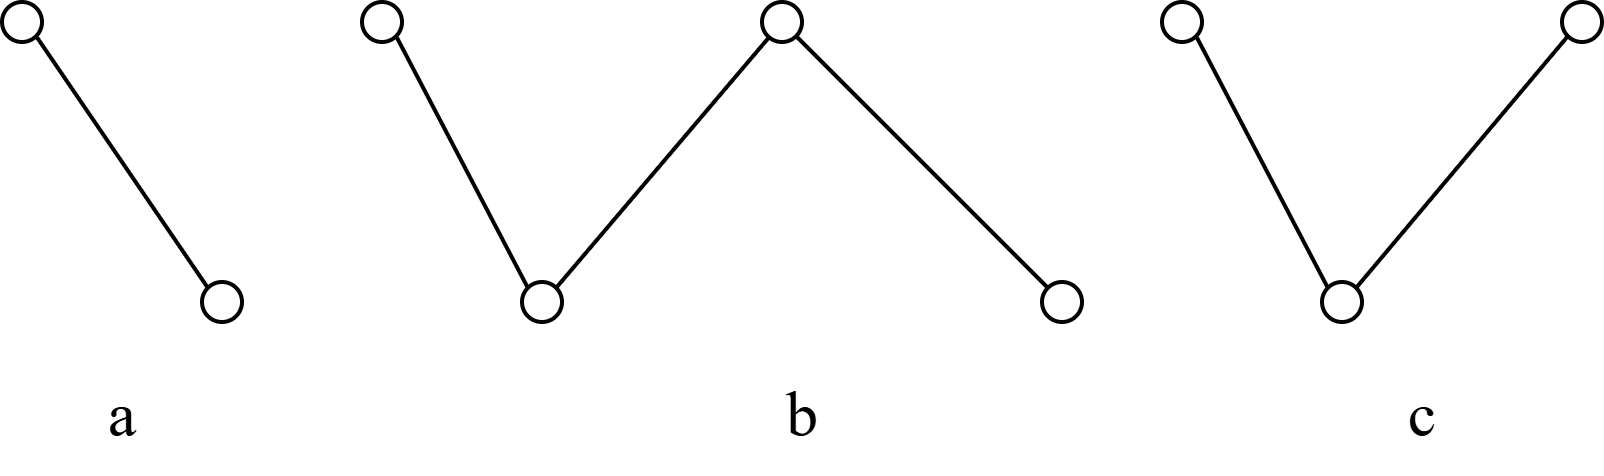
\includegraphics[width=0.8\textwidth]{images/1-1-1.png}
  \caption{Rigid Body}
  \label{fig:1-1-1}
\end{figure}

\subsection{Degrees of Freedom}

\begin{definition}[Degrees of Freedom]
    Number of variables required to uniquely specify the system.
\end{definition}

For example, if we have a 3D object which consists of $M$ moving parts, then we have:

\[
    \text{\# degrees of freedom} = 3M -N
\]

where $N$ is the number of constraints in this system.

Let's take a look at the Figure \ref{fig:1-1-1}. For a, 

\[
    \text{\# degrees of freedom} = 3 \times 2 - 1 = 5 \ \text{DOF}
\]

For b (all angles are fixed),

\[
    \text{\# degrees of freedom} = 3 \times 4 - 3 \ \text{lengths} - 3 \ \text{angles} = 3 \ \text{COM} + 3 \ \text{orientations} = 6 \ \text{DOF}
\]

For c (the angle is not fixed),

\[
    \text{\# degrees of freedom} = 3 \times 3 - 2 \ \text{lengths} = 7 \ \text{DOF}
\]

What needs to be noticed is that dynamic variables don't have to be the usual Cartesian coordinates.

\[
    \mathbf{r} = (x, y, z) = (r, \theta, \phi) ...
\]

\begin{figure}[h]
  \centering
  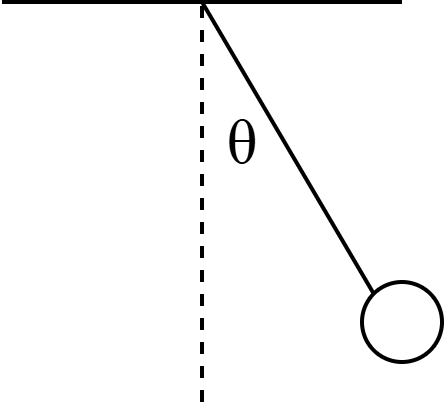
\includegraphics[width=0.8\textwidth]{images/1-1-2.png}
  \caption{Pendulum Example}
  \label{fig:1-1-2}
\end{figure}

Consider the pendulum example in Figure \ref{fig:1-1-2}. There is only $1$ DOF, so you can choose $x$, $y$, or $\theta$ to depict the motion of the pendulum.

Let's introduce the concept of Generic Degrees of Freedom $q_i, i=1, 2, ..., N$, where $N$ is the number of degrees of freedom. In this way, for a constrained system, the position of any part of the system will be a function of $q_i$.

\[
    \mathbf{r}_\alpha = \mathbf{r}_\alpha(q_i, t),\ \alpha=\text{\# parts}
\]

Here we allow any part of the system to have explicit dependence on time. If we can write $\mathbf{r}_\alpha(q_i, t)$ for a system, then the system (or sometimes we say the constraints of the system) is \textbf{holonomic}. Otherwise, the system is  \textbf{nonholonomic}. For these systems, if the relations are time independent, then the system is \textbf{scleronomic}. Otherwise, the system is \textbf{rheonomic}. 

\begin{figure}[h]
  \centering
  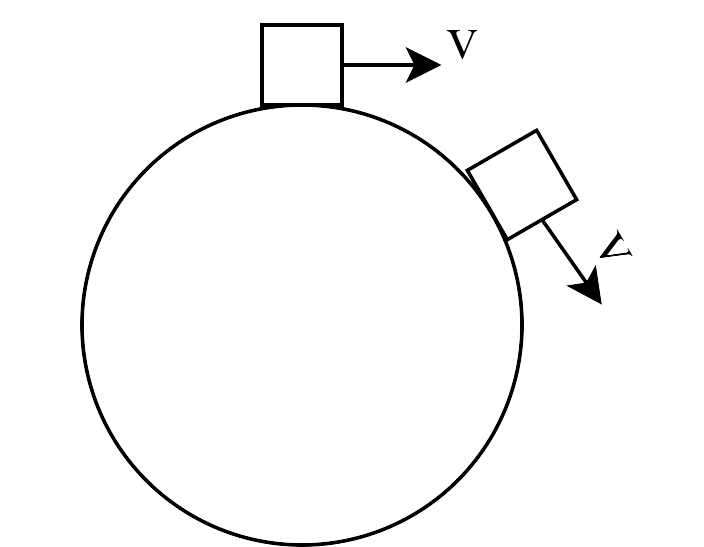
\includegraphics[width=0.8\textwidth]{images/1-1-3.png}
  \caption{Rigid Body}
  \label{fig:1-1-3}
\end{figure}

Nonholonomic systems are common in the real world. Consider the example in Figure \ref{fig:1-1-3}, where DOF changes from $2$ to $3$ if the box flies free.

\subsection{Lagrangian Mechanics}

Consider a dynamical system $q_i, i=1,2,..,\text{\# DOF}$. For a typical mechanical system, the positions of the various parts can be written as $\mathbf{r}_\alpha=\mathbf{r}_\alpha(q_i, t)$, and the basic problem for this system is to determine the $q_i(t)$. $q_i(t)$ satisfy a system of $N$ differential equations known as \textbf{Equations of Motions}.

In the past, we typically used the old way of Newton's Law, which requires constraint forces:

\begin{enumerate}
    \item Determine the force $F_\alpha$ on a part of the system $r_\alpha$
    \item Use the $2^{\text{nd}}$ order ordinary differential equations (ODEs) for $r_\alpha$: 
    \[
        \mathbf{F}_\alpha = m \ddot{\mathbf{r}}_\alpha
    \]
    \item Rewrite $\mathbf{r}_\alpha$ in terms of $q_i$, and we can get $2^{\text{nd}}$ order ODEs for $\mathbf{r}_\alpha$, which is easier to said than done!
\end{enumerate}

Now we need to come up with a way to eliminate the need to use constraint forces: \textbf{Lagrangian Mechanics}!

If we change $\mathbf{r}_\alpha$ to $\mathbf{r}_\alpha+\delta \mathbf{r}_\alpha$, then the work done is:

\[
   \delta W = \sum_{\alpha} \mathbf{F}_\alpha \delta \mathbf{r}_\alpha
\]

This raises a question: how much work is done if we change $q_i$ to $q_i+\delta q_i$? Since $\mathbf{r}_\alpha = \mathbf{r}_\alpha(q_i, t)$, we can get (here we only consider one degree of freedom):

\[
   \mathbf{r}_\alpha = \sum_{i} \frac{\partial \mathbf{r}_\alpha}{\partial q_i} \delta q_i
\]

\begin{align*}
    \delta W &= \sum_{\alpha} \mathbf{F}_\alpha \left(\sum_{i} \frac{\partial \mathbf{r}_\alpha}{\partial q_i} \delta q_i \right) \\
             &= \sum_{i} \left(\sum_{\alpha} \mathbf{F}_{\alpha} \frac{ \partial \mathbf{r}_\alpha}{\partial q_i} \right) \delta q_i
\end{align*}

\[
   \sum_{\alpha} \mathbf{F_{\alpha}} \frac{\partial \mathbf{r}_\alpha}{\partial q_i} = F_i
\]

Here we call $F_i$ a \textbf{generalized force} associated with the variable $q_i$, and $F_i$ is the force in the "allowed directions". 

Now let's discuss the kinetic energy of a constrained system:

\begin{align*}
    T &= \frac{1}{2} \sum_{\alpha} m_\alpha \dot{\mathbf{r}}_\alpha \cdot \dot{\mathbf{r}}_\alpha \\
      &= T(q_i, \dot{q_i}, t) \\
\end{align*}

\begin{align*}
    \mathbf{r}_\alpha &= \mathbf{r}_\alpha(q_i, t) \\
    \dot{\mathbf{r}}_\alpha &= \sum_i \frac{\partial \mathbf{r}_\alpha}{q_i} \dot{q_i} + \frac{\partial \mathbf{r}_\alpha}{t}
\end{align*}

Since:

\[
    \frac{\partial \dot{\mathbf{r}}_\alpha}{\dot{q_i}} = \frac{\partial \mathbf{r}_\alpha}{q_i}
\]

We can get:

\begin{align*}
    \frac {\partial T}{\partial q_i} &= \sum_\alpha m_\alpha \dot{\mathbf{r}}_\alpha \frac{\partial \dot{\mathbf{r}}_\alpha}{\partial q_i} \\
    \frac {\partial T}{\partial \dot{q_i}} &= \sum_\alpha m_\alpha \dot{\mathbf{r}}_\alpha \frac{\partial \dot{\mathbf{r}}_\alpha}{\partial \dot{q_i}} = \sum_\alpha m_\alpha \dot{\mathbf{r}}_\alpha \frac{\partial \mathbf{r}_\alpha}{\partial q_i}\\
\end{align*}

Therefore, 

\begin{align*}
    \frac{d}{dt} (\frac {\partial T}{\partial \dot{q_i}}) &= \sum_\alpha m_\alpha \left(\ddot{\mathbf{r}}_\alpha \frac{\partial \mathbf{r}_\alpha}{\partial q_i} + \dot{\mathbf{r}}_\alpha \frac{\partial \dot{\mathbf{r}}_\alpha}{\partial q_i}\right) \\
    &= \sum_\alpha \mathbf{F}_\alpha \frac{\partial \mathbf{r}_\alpha}{\partial q_i} + \frac{\partial T}{\partial q_i} \\
    &= \mathbf{F}_i + \frac{\partial T}{\partial q_i} \\
\end{align*}

So we can get:

\[
    \mathbf{F}_i = \frac{d}{dt} (\frac {\partial T}{\partial \dot{q_i}}) - \frac{\partial T}{\partial q_i}
\]

If we know $T(q_i, \dot{q}_i, t)$, we can write down the generalized force without computing a constraint! We can get a generalization of $\mathbf{F}=m\mathbf{a}$ to a generic degree of freedom!